\chapter{Zadanie 2}
	\label{ch:zadanie2}
	
	\section{Obiekt rozmyty}
		\label{sec:ob_roz}
		Utworzenie modelu rozmytego Takagi-Sugeno dla obiektu należy zacząć od wyznaczenia funkcji przynależności. Jako funkcji przynależności zdecydowaliśmy się użyć funkcji sigmoidalnych. Ponieważ projekt zakłada utworzenie modeli rozmytych z dwoma, trzema, czterema oraz pięcioma modelami lokalnymi, funkcje przynależności dla pierwszego, n-tego oraz ostatniego (przy r obecnych modelach lokalnych) modelu lokalnego wyglądają tak jak w równaniach od \ref{eq:sig1} do \ref{eq:sigost}. W podanych wzorach zmienna a oznacza nachylenie funkcji i została przyjęta taka sama dla wszystkich modeli lokalnych. Wektor c natomiast zawiera punkty dla których funkcje przynależności sąsiednich modeli lokalnych osiągają wartość 0.5. Wartość a została dobrana eksperymentalnie na poziomie a=3. Wartości c zostały wyliczone poprzez podzielenie zakresu wartości zmiennej na podstawie której liczony jest obiekt rozmyty przez ilość regulatorów lokalnych, co zagwarantowało w równomierny podział zbiorów rozmytych. Zdecydowaliśmy się na wykorzystanie wyjścia obiektu jako zmiennej determinującej zbiory rozmyte. Decyzja ta poparta była faktem, że dla sterowania w obiekcie występuje znaczne opóźnienie co prawdopodobnie uniemożliwiłoby późniejsze zaimplementowanie na utworzonych zbiorach rozmytych skutecznie działającego regulatora. Dla badanego w zadaniu pierwszym zakresu sterowań wyjście obiektu przyjmuje wartości w przybliżeniu od 4.5 do 34.5, dlatego właśnie w takim zakresie tworzone były zbiory rozmyte. Dodatkowo dla każdego zbioru rozmytego należało określić punkt pracy w którym zlinearyzowany był obiekt lokalny. Punkty pracy zostały wyznaczone na podstawie kształtu poszczególnych funkcji przynależności. Wartość wyjścia w punkcie pracy dla wybranego modelu równa jest w przybliżeniu wartości wyjścia znajdującej się w środku przedziału dla którego funkcja przynależności wynosi 1. Funkcje przynależności dla utworzonych obiektów rozmytych przedstawione zostały na wykresach od \ref{rys:roz2} do \ref{rys:roz5}.
		
		\begin{equation}
			\mu(1) = 1-\frac{1}{1+e^{-a*(h2-c(1))}}
			\label{eq:sig1}
		\end{equation}
		\begin{equation}
			\mu(n) = \frac{1}{1+e^{-a*(h2-c(n-1))}}-\frac{1}{1+e^{-a*(h2-c(n))}}
			\label{eq:sign}
		\end{equation}
		\begin{equation}
		\mu(r) = \frac{1}{1+e^{-a*(h2-c(r-1))}}
		\label{eq:sigost}
		\end{equation}
		
		\begin{figure}[h!]
			\includegraphics[width=0.9\linewidth]{plots/z2_modelroz_2.eps}
			\caption{Funkcje przynależności dla obiektu rozmytego z dwoma obiektami lokalnymi}
			\label{rys:roz2}
		\end{figure}
		\begin{figure}[h!]
			\includegraphics[width=0.9\linewidth]{plots/z2_modelroz_3.eps}
			\caption{Funkcje przynależności dla obiektu rozmytego z trzema obiektami lokalnymi}
			\label{rys:roz3}
		\end{figure}
		\begin{figure}[h!]
			\includegraphics[width=0.9\linewidth]{plots/z2_modelroz_4.eps}
			\caption{Funkcje przynależności dla obiektu rozmytego z czterema obiektami lokalnymi}
			\label{rys:roz4}
		\end{figure}
		\begin{figure}[h!]
			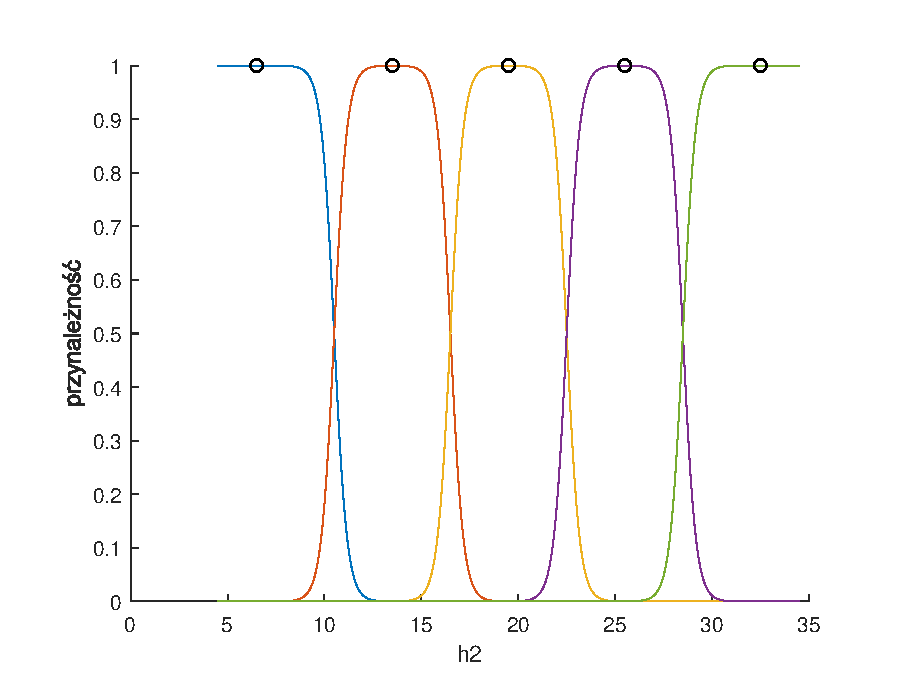
\includegraphics[width=0.9\linewidth]{plots/z2_modelroz_5.eps}
			\caption{Funkcje przynależności dla obiektu rozmytego z pięcioma obiektami lokalnymi}
			\label{rys:roz5}
		\end{figure}
	
	
		Utworzenie obiektu rozmytego na podstawie przedstawionych funkcji przynależności nie sprawiło już zbytniego problemu. Zakładając, że obiekt ma określoną ilość zbiorów rozmytych i każdy zbiór posiada swój punkt linearyzacji zaimplementowane została określona ilość obiektów liniowych. W każdej iteracji liczone są wyjścia wszystkich obiektów liniowych oraz wagi według funkcji przynależności. Następnie faktyczny stan obiektu otrzymywany jest poprzez przemnożenie wyników lokalnych przez ich wagi i podzielenie otrzymanej liczby przez sumę wag. Oczywiście dla każdego modelu liniowego potrzebny jest punkt linearyzacji, który jak już wspominałem został określony jedynie poprzez wartość wyjścia obiektu $h_{20}$. Wartości $V_{10}$, $V_{20}$ oraz $h_{10}$ obliczane są analogicznie jak dla obiektu liniowego z pierwszego zadania. Co do wartości zakłócenia $F_{D0}$ ustalona została ona na 10. Wartość sterowania w punkcie linearyzacji $F_{10}$ można zatem wyliczyć podstawiając wartość 0 pod pochodną $dV/dt$, co daje nam działanie $F_{10} = \alpha_1*\sqrt{h_{20}}-F_{D0}$.
		
		Porównania działania poszczególnych modeli rozmytych modelem nieliniowym oraz liniowym obiektu przedstawione zostały na wykresach od \ref{rys:roz2p} do \ref{rys:roz5p}. Dla każdego modelu wykonane zostały przebiegi ze skokami sterowania w kroku 100. Użyte skoki sterowania są takie same jak w zadaniu pierwszym. Na wykresach przebiegi dla oryginalnego obiektu przedstawione są kolorem niebieskim, dla zlinearyzowanego różowym, a dla rozmytego zielonym.
		
		Dla modelu z dwoma obiektami lokalnymi działanie modelu rozmytego definitywnie nie jest zadowalające. Końcowa wartość wyjścia obiektu rozmytego w większości przypadków zauważalnie rozbiega się z końcową wartością dla oryginalnego modelu. Kształty przebiegów dla poszczególnych skoków nie są podobne do przebiegów nieliniowego ani liniowego obiektu. Przebiegiem, który najbardziej pokrywa się z oryginałem jest ten dla skoku sterowania do 34 (drugi od dołu).
		
		Dla modelu z trzema obiektami lokalnymi sytuacja wydaje się lepsza. Przebiegi dla skoków powyżej punktu pracy są zbliżone w wyglądzie do oryginalnego obiektu. Nie licząc przebiegu dla skoku sterowania do 24 (pierwszy od dołu) wartości końcowe wyjścia obiektu rozmytego w przybliżeniu pokrywają się z wartościami dla obiektu oryginalnego.
		
		Dla modelu z czterema obiektami lokalnymi znowu nastąpiła nieznaczna poprawa. Przebiegi przez większość symulacji pokrywają się kształtem z przebiegami dla pierwotnego modelu, jednakże część wartości końcowych wyjścia nieznacznie odbiega od pożądanych.

		Modelu z pięcioma obiektami lokalnymi działa najlepiej z przedstawionych. Poza kilkoma miejscami przebiegi pokrywają się z przebiegami dla oryginalnego obiektu. Wartości końcowe także są w przybliżeniu równe wartościom końcowym dla obiektu oryginalnego. Obiekt ten jest zdecydowanie najlepszym z utworzonych i to właśnie on wykorzystywany będzie do dalszych badań.
		
		\begin{figure}[h!]
			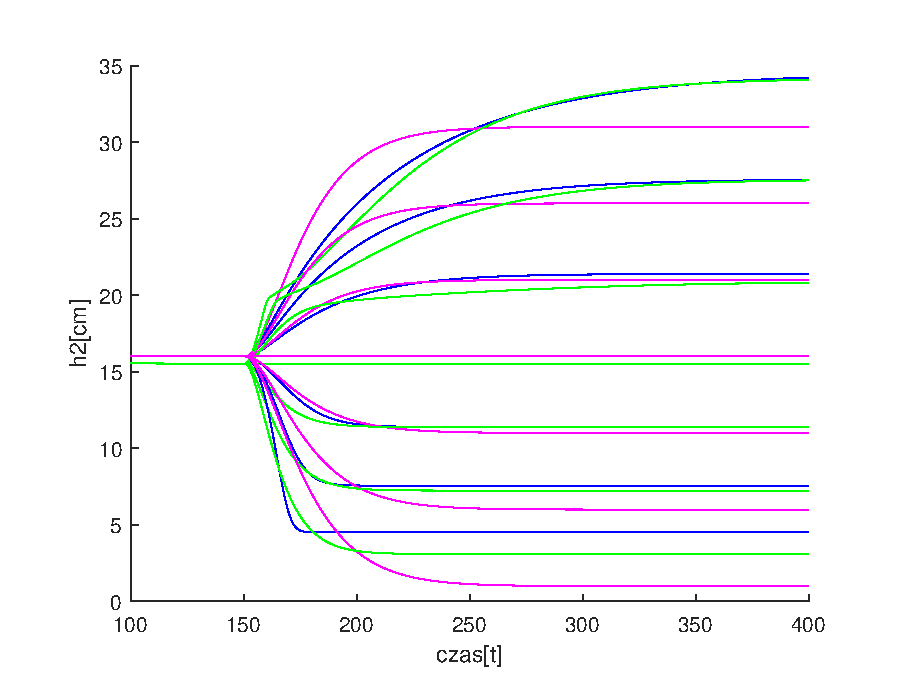
\includegraphics[width=0.9\linewidth]{plots/z2_modelroz_2p.eps}
			\caption{Porównanie działania dla obiektu rozmytego z dwoma obiektami lokalnymi}
			\label{rys:roz2p}
		\end{figure}
		\begin{figure}[h!]
			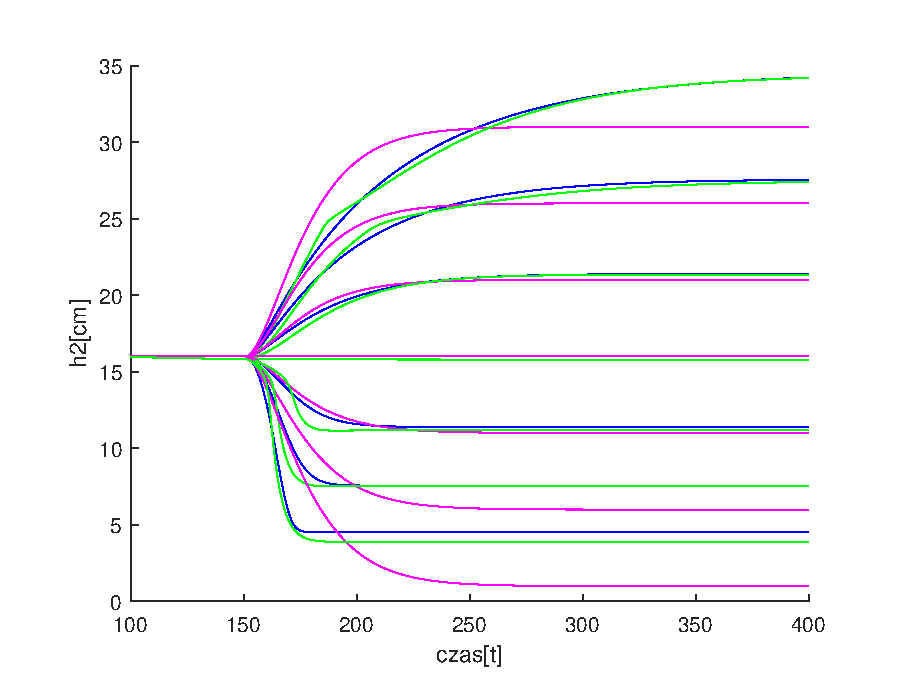
\includegraphics[width=0.9\linewidth]{plots/z2_modelroz_3p.eps}
			\caption{Porównanie działania dla obiektu rozmytego z trzema obiektami lokalnymi}
			\label{rys:roz3p}
		\end{figure}
		\begin{figure}[h!]
			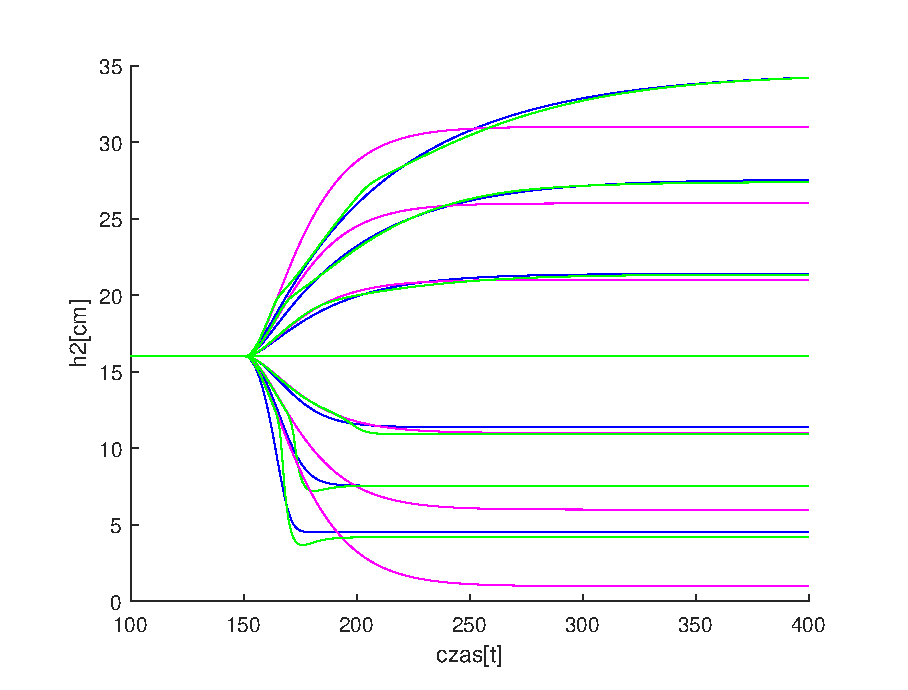
\includegraphics[width=0.9\linewidth]{plots/z2_modelroz_4p.eps}
			\caption{Porównanie działania dla obiektu rozmytego z czterema obiektami lokalnymi}
			\label{rys:roz4p}
		\end{figure}
		\begin{figure}[h!]
			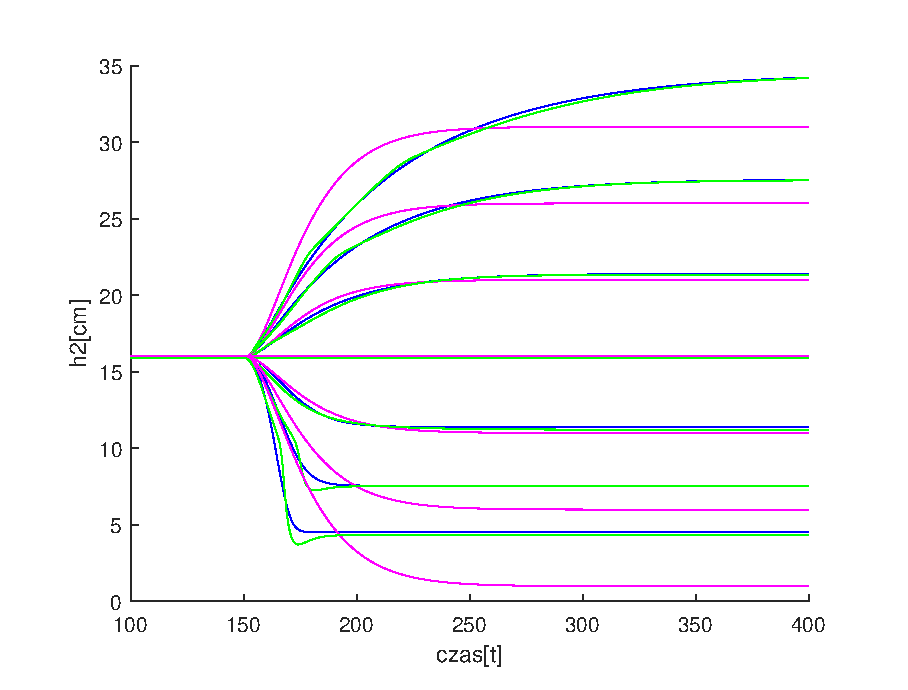
\includegraphics[width=0.9\linewidth]{plots/z2_modelroz_5p.eps}
			\caption{Porównanie działania dla obiektu rozmytego z pięcioma obiektami lokalnymi}
			\label{rys:roz5p}
		\end{figure}
	\newpage
	\section{DMC rozmyty}
	%z2_dmcroz(400, 400, 400, 400, 2000,[],[], true)
	dmc oryginalny - 18.2898
	%z2_dmcroz(400, 400, 400, 400, 2000,10,[8.5000   17.5000   24.5000   33.5000], true)
	dmc zmiana rozmycia - 18.2504
	%z2_dmcroz(400, 400, 400, 400, 100,10,[8.5000   17.5000   24.5000   33.5000], true)
	dmc lambda 100 - 13.6096
	%z2_dmcroz(200, 150, 100, 200, 100,10,[8.5000   17.5000   24.5000   33.5000], true)
	dmc mniejsze horyzonty - 13.5395
		